\documentclass[]{book}
\usepackage{lmodern}
\usepackage{amssymb,amsmath}
\usepackage{ifxetex,ifluatex}
\usepackage{fixltx2e} % provides \textsubscript
\ifnum 0\ifxetex 1\fi\ifluatex 1\fi=0 % if pdftex
  \usepackage[T1]{fontenc}
  \usepackage[utf8]{inputenc}
\else % if luatex or xelatex
  \ifxetex
    \usepackage{mathspec}
  \else
    \usepackage{fontspec}
  \fi
  \defaultfontfeatures{Ligatures=TeX,Scale=MatchLowercase}
\fi
% use upquote if available, for straight quotes in verbatim environments
\IfFileExists{upquote.sty}{\usepackage{upquote}}{}
% use microtype if available
\IfFileExists{microtype.sty}{%
\usepackage{microtype}
\UseMicrotypeSet[protrusion]{basicmath} % disable protrusion for tt fonts
}{}
\usepackage{hyperref}
\hypersetup{unicode=true,
            pdftitle={e-Business},
            pdfauthor={Robert Batzinger},
            pdfborder={0 0 0},
            breaklinks=true}
\urlstyle{same}  % don't use monospace font for urls
\usepackage{natbib}
\bibliographystyle{apalike}
\usepackage{longtable,booktabs}
\usepackage{graphicx,grffile}
\makeatletter
\def\maxwidth{\ifdim\Gin@nat@width>\linewidth\linewidth\else\Gin@nat@width\fi}
\def\maxheight{\ifdim\Gin@nat@height>\textheight\textheight\else\Gin@nat@height\fi}
\makeatother
% Scale images if necessary, so that they will not overflow the page
% margins by default, and it is still possible to overwrite the defaults
% using explicit options in \includegraphics[width, height, ...]{}
\setkeys{Gin}{width=\maxwidth,height=\maxheight,keepaspectratio}
\IfFileExists{parskip.sty}{%
\usepackage{parskip}
}{% else
\setlength{\parindent}{0pt}
\setlength{\parskip}{6pt plus 2pt minus 1pt}
}
\setlength{\emergencystretch}{3em}  % prevent overfull lines
\providecommand{\tightlist}{%
  \setlength{\itemsep}{0pt}\setlength{\parskip}{0pt}}
\setcounter{secnumdepth}{5}
% Redefines (sub)paragraphs to behave more like sections
\ifx\paragraph\undefined\else
\let\oldparagraph\paragraph
\renewcommand{\paragraph}[1]{\oldparagraph{#1}\mbox{}}
\fi
\ifx\subparagraph\undefined\else
\let\oldsubparagraph\subparagraph
\renewcommand{\subparagraph}[1]{\oldsubparagraph{#1}\mbox{}}
\fi

%%% Use protect on footnotes to avoid problems with footnotes in titles
\let\rmarkdownfootnote\footnote%
\def\footnote{\protect\rmarkdownfootnote}

%%% Change title format to be more compact
\usepackage{titling}

% Create subtitle command for use in maketitle
\providecommand{\subtitle}[1]{
  \posttitle{
    \begin{center}\large#1\end{center}
    }
}

\setlength{\droptitle}{-2em}

  \title{e-Business}
    \pretitle{\vspace{\droptitle}\centering\huge}
  \posttitle{\par}
    \author{Robert Batzinger}
    \preauthor{\centering\large\emph}
  \postauthor{\par}
      \predate{\centering\large\emph}
  \postdate{\par}
    \date{2019-06-20}

\usepackage{booktabs}
\usepackage{amsthm}
\usepackage{graphicx}
\makeatletter
\def\thm@space@setup{%
  \thm@preskip=8pt plus 2pt minus 4pt
  \thm@postskip=\thm@preskip
}
\makeatother

\newenvironment{rmdexercise}{$$\begin{minipage}[t]{1cm}\vbox to 0pt{\null\kern 5pt\hbox{
\includegraphics[width=1cm]{images/checklist.png}}\vss}\end{minipage}\quad
   \begin{minipage}[t]{4.25in}\hrule\smallskip\small}{\smallskip\hrule\end{minipage}$$}
\newenvironment{rmdextra}{$$\begin{minipage}[t]{1cm}\vbox to 0pt{\null\kern 5pt\hbox{
\includegraphics[width=1cm]{images/study.png}}\vss}\end{minipage}\quad
   \begin{minipage}[t]{4.25in}\hrule\smallskip\small}{\smallskip\hrule\end{minipage}$$}
\newenvironment{rmddiscussion}{$$\begin{minipage}[t]{1cm}\vbox to 0pt{\null\kern 5pt\hbox{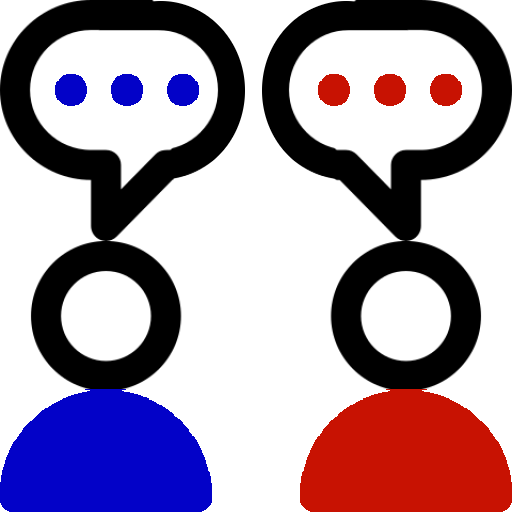
\includegraphics[width=1cm]{images/discuss.png}}\vss}\end{minipage}\quad
   \begin{minipage}[t]{4.25in}\hrule\smallskip\small}{\smallskip\hrule\end{minipage}$$}

\let\BeginKnitrBlock\begin \let\EndKnitrBlock\end
\begin{document}
\maketitle

{
\setcounter{tocdepth}{1}
\tableofcontents
}
\hypertarget{book-jacket}{%
\chapter*{Book Jacket}\label{book-jacket}}
\addcontentsline{toc}{chapter}{Book Jacket}

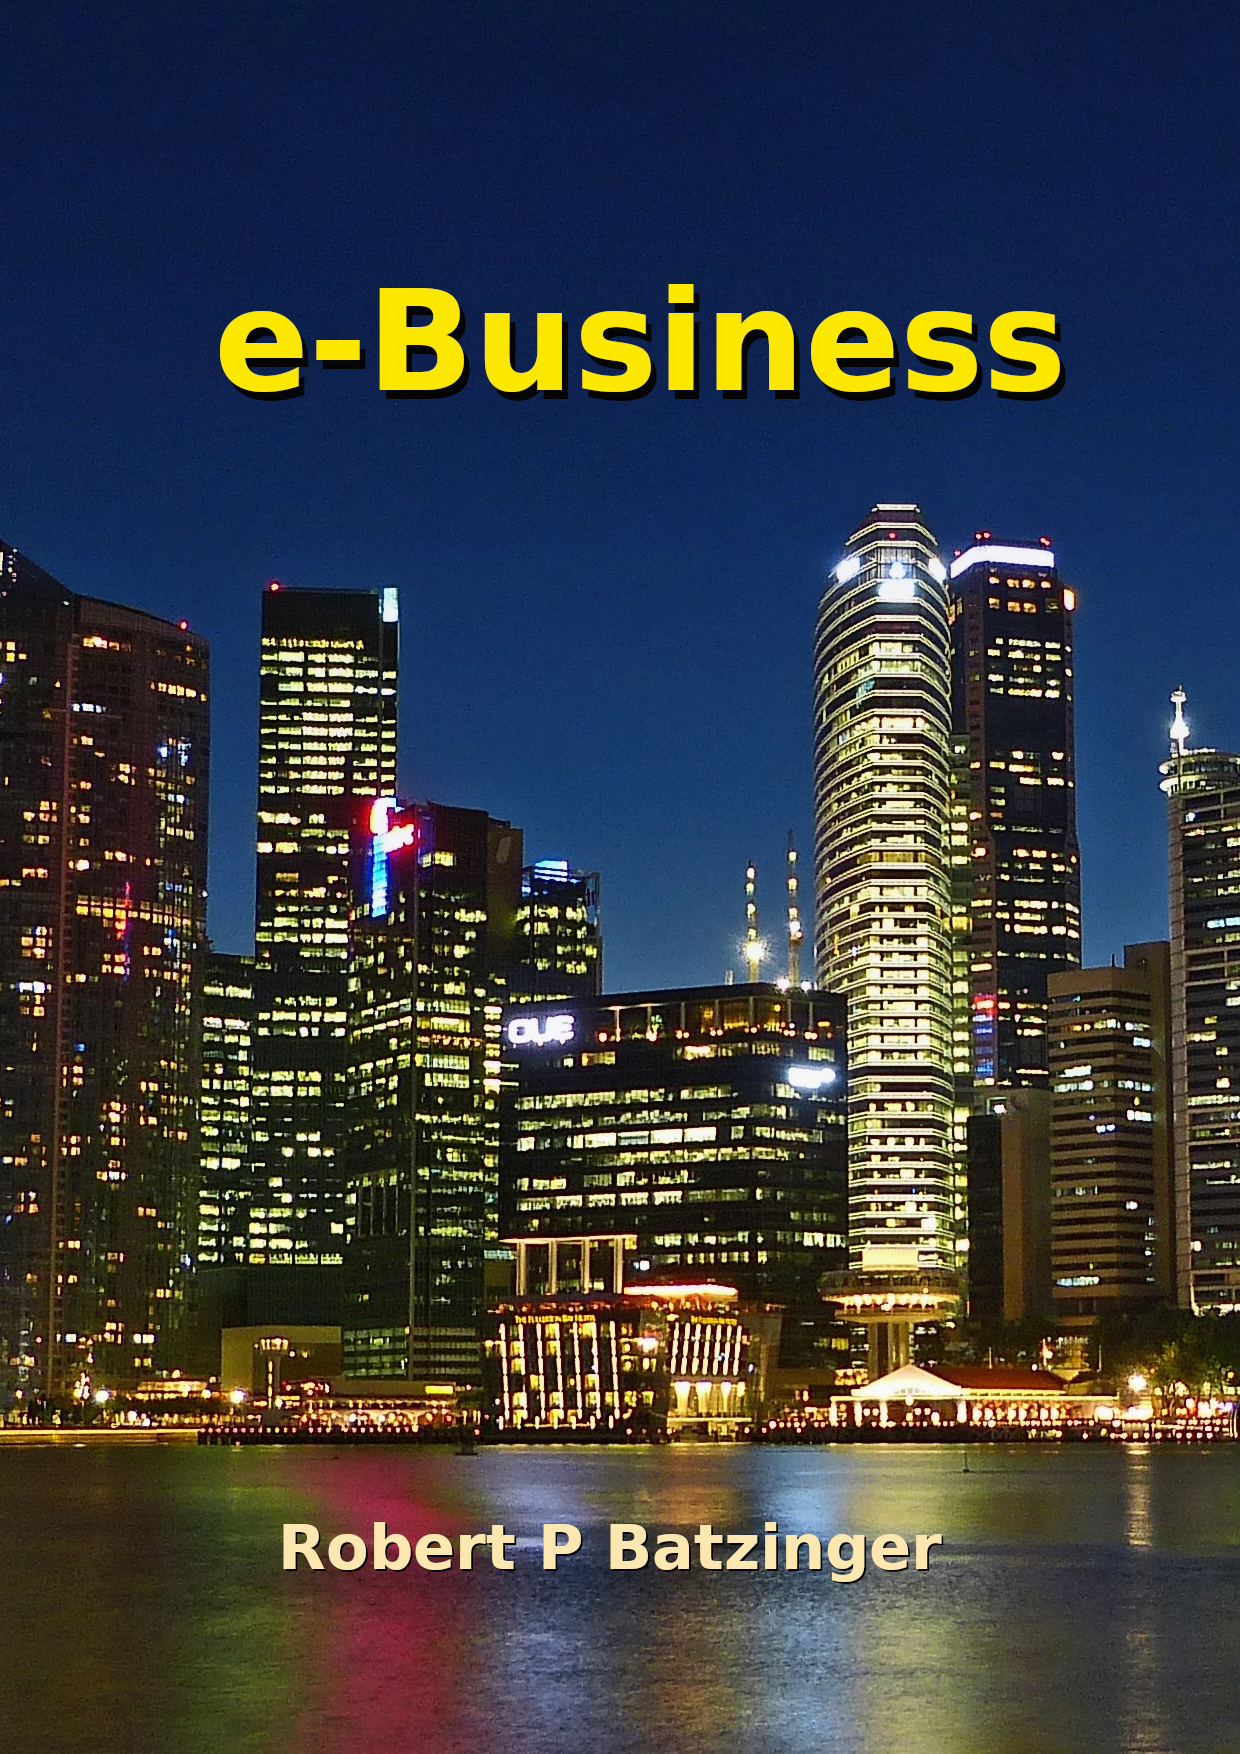
\includegraphics[width=0.5\linewidth]{images/cover11}

\hypertarget{abstract}{%
\section*{Abstract}\label{abstract}}
\addcontentsline{toc}{section}{Abstract}

This book attempts to introduce undergraduate students to the nature and requirements for conducting business online. It starts with a discussion of the nature of business and the challenges and potential of the online environment, followed by a review of common methods of modelling business, and a study of open source business solutions.
The final chapter focuses on emerging trends and sea-changes in e-Business. This book is currently a work in progress that is also comparing the process of book writing in both LeanPub markdown and Rstudio Bookdown

\hypertarget{about-the-author}{%
\section*{About the Author}\label{about-the-author}}
\addcontentsline{toc}{section}{About the Author}

Robert Batzinger is an emeritus instructor in Computer Science at Payap University. He holds an undergraduate degree in Organic Chemistry, masters degree in Computer Science and Applied Mathematics, doctoral degree in Pathobiology and post-doctoral training in Chemical carcinogenesis. As such, he has been involved in numerous scientific and technical projects for over 50 years. He has published laboratory research in such fields as virology, organic chemistry, anthelmithics, and chemical mutagenesis. He also developed software to manage the financial and academic records of schools, support the development of publications in non-Roman scripts of Asia and Canada, and monitor the progress of multiple development projects. He has held administrative and advisory roles in various organizations and businesses, and has been instrumental in establishing web presence for many of them. He is currently developing data science and machine learning applications to address critical business management problems.

\hypertarget{front-matter}{%
\chapter*{Front Matter}\label{front-matter}}
\addcontentsline{toc}{chapter}{Front Matter}

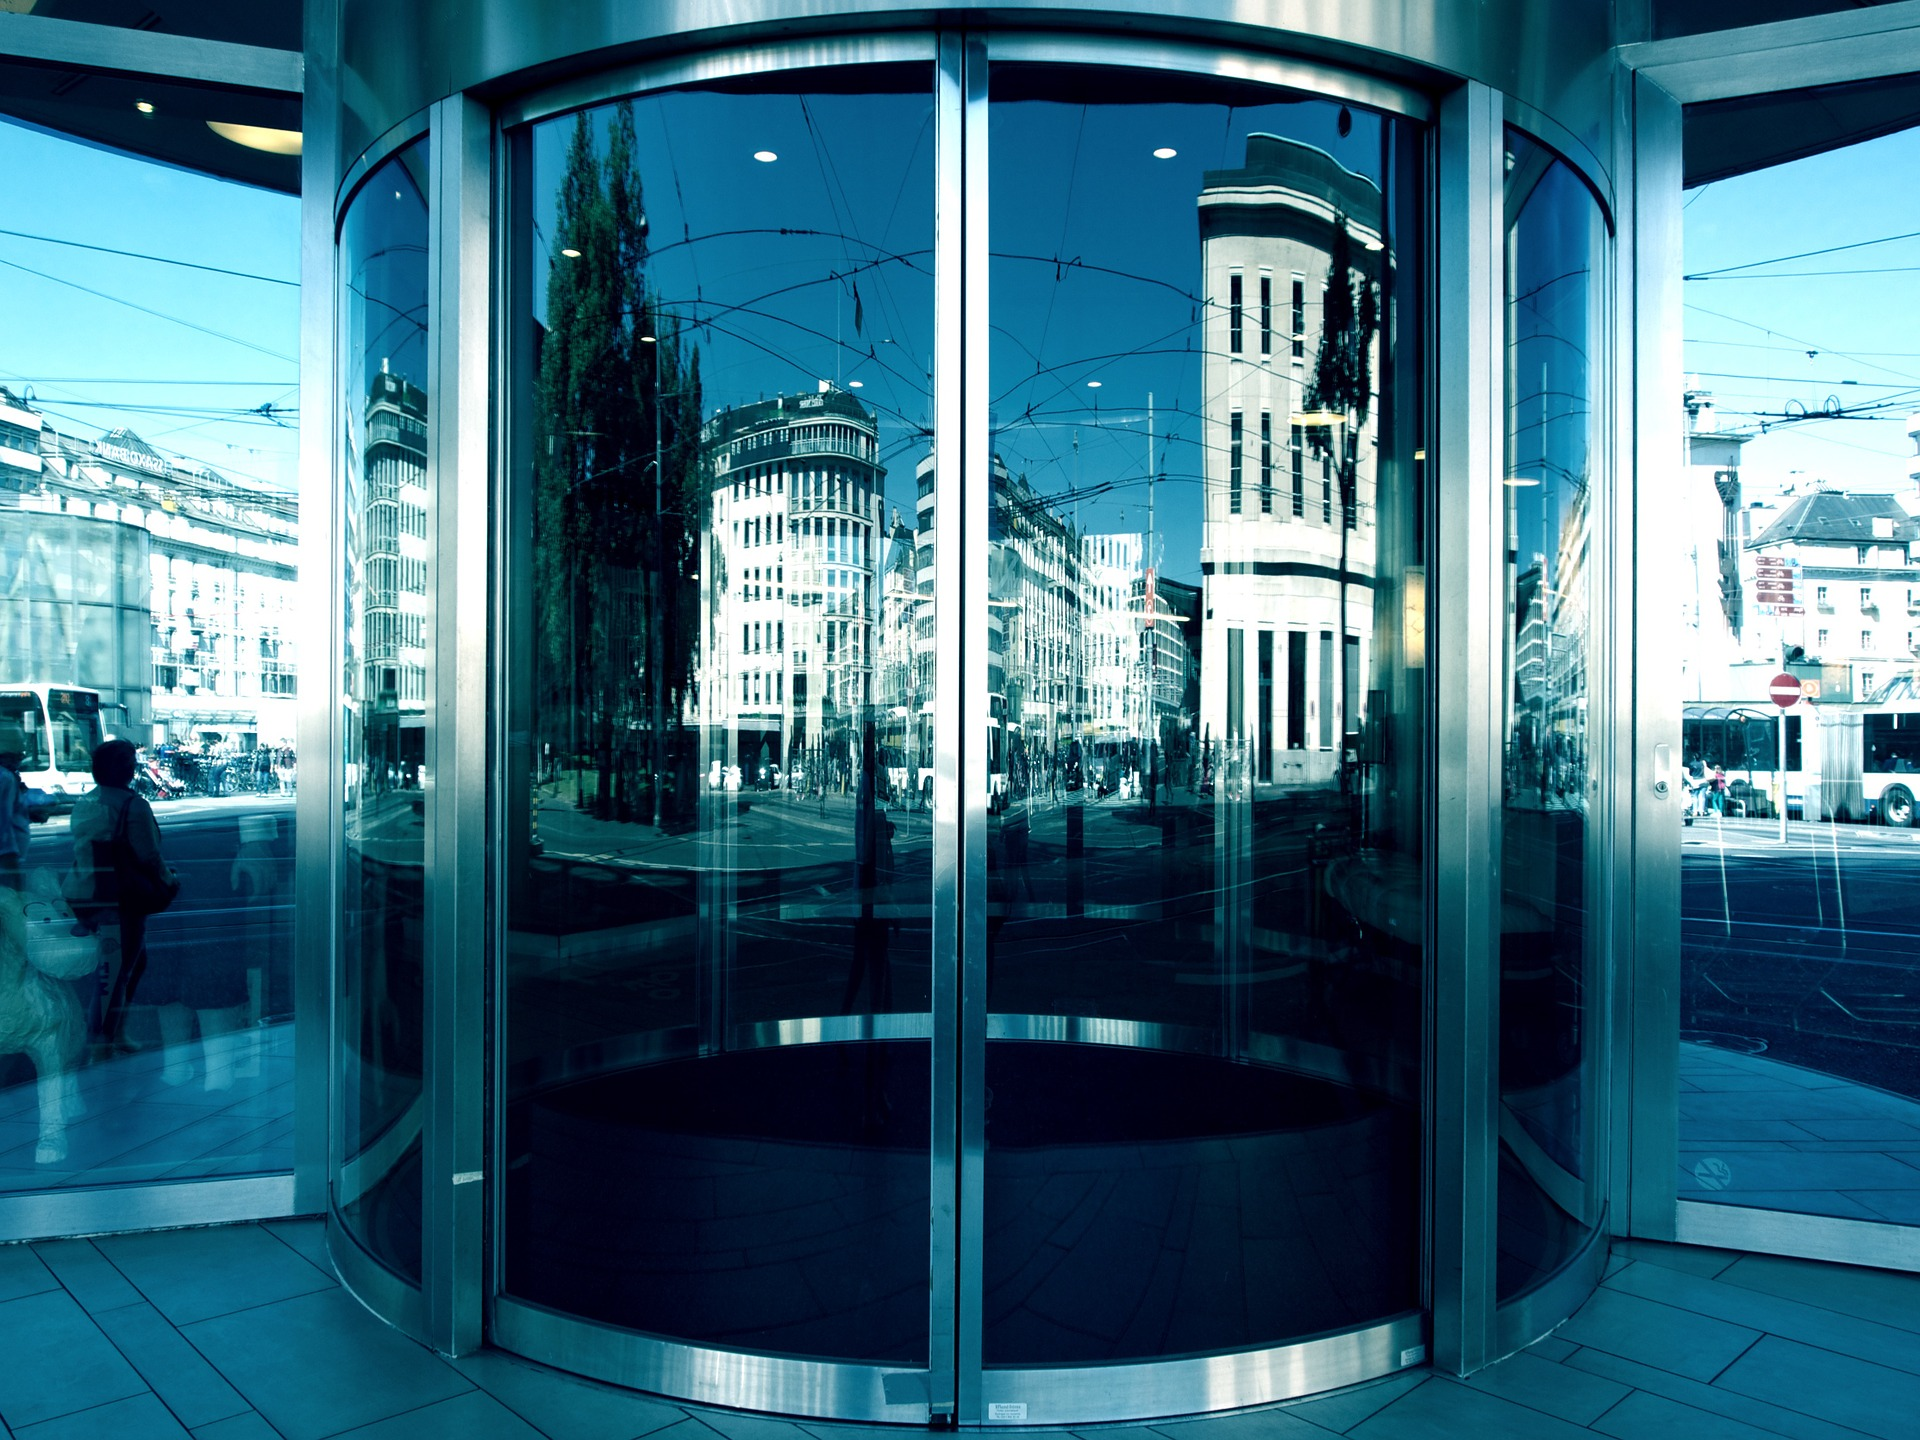
\includegraphics[width=0.9\linewidth]{images/door}

\hypertarget{dedication}{%
\section*{Dedication}\label{dedication}}
\addcontentsline{toc}{section}{Dedication}

\begin{quote}
Now to him who is able to do far more abundantly
than all that we ask or think, according
to the power at work within us.
-- Eph 3:20 (ESV)

ขอให้พระเกียรติมีแด่พระองค์ผู้ทรงสามารถทำทุกสิ่งได้
มากยิ่งกว่าที่เราทูลขอหรือคิด โดยฤทธานุภาพ
ที่ทำกิจอยู่ภายในเรา
-- เอเฟซัส 3:20 (THSV11)
\end{quote}

\hypertarget{acknowledgements}{%
\section*{Acknowledgements}\label{acknowledgements}}
\addcontentsline{toc}{section}{Acknowledgements}

The development of this book would not have been possible without the feedback and suggestions of colleagues and students. While I acknowledge that I am responsible for any remaining errors in this book, my students, referees, and readers have contributed immensely to the development of this book. I would like to acknowledge the impact of Ms.~Phatnaree Srisomphan in helping to shape both the curriculum of this course and the nature of this book. I am also grateful for the support and encouragement of my wife Khajohn, especially in those long critical sessions when I was struggling to forge and edit the text of this manuscript.

\hypertarget{colophon}{%
\section*{Colophon}\label{colophon}}
\addcontentsline{toc}{section}{Colophon}

The cover is a photograph of the Financial District from the Marina Bay in Singapore. The amazing metamorphsis of this central business district from swamp land into a thriving financial center of the Region is representative of the current sea-changes in business driven by technological and social developments. Similarly, today's developers of business systems are sowing seeds that will change the future, much like Sir Raffles' vision for a seaport has grown into today's Singapore.

While early drafts of this book were written in Leanpub Flavored Markdown, this book was developed in RStudio using the \textbf{bookdown} package \citep{R-bookdown} (which was built on top of R Markdown and \textbf{knitr} \citep{xie2015}. It was compiled in RStudio and published simultaneously as an HTML website, a printable document in PDF and electronic book EPUB format.

The cover and front matter photos were downloaded from \href{https://pixabay.com/images/search/singapore}{Pixabay}.
The extra reading, discussion and exercise sidebar icons were created by \href{https://www.freepik.com}{Freepik} and used as per \href{https://creativecommons.org/licenses/by/3.0}{Creative Commons 3.0 License}.

\hypertarget{preface}{%
\chapter*{Preface}\label{preface}}
\addcontentsline{toc}{chapter}{Preface}

Advances and developments in Computer Science (CS) are driven by the need to create applications that effectively address real-world problems. Successful software development starts with a deep understanding of the problem domain from the users perspective and developing an application that is intuitive and easy to use. Breakthroughs in understanding the nature of a problem domain create new opportunities for addressing the needs of computer users. It is now common practice to integrate end users into software development and testing teams, as the resulting products tend to be more intuitive and successful.

In CS, our graduates will go on to develop applications and solutions for clients who, for the most part, have not studied CS, but who are experts in other problem domains. Courses that help students to explore and understand the basic issues in other problem domains are at the heart of our liberal arts education which balances professional skills with general knowledge needed to function effectively in the market place.
As a part of this effort to introduce CS students to e-Business from a Business/IT perspective, we offer a course with the following course description. It is taught in Thai using English-based resources.

\begin{quote}
\textbf{CS340 ธุรกิจอิเล็กทรอนิกส์:} หลักการการดำเนินธุรกิจโดยใช้สื่ออิเล็กทรอนิกส์ การวางแผนทรัพยากรขององค์กร การบริหารความสัมพันธ์ลูกค้า และการสื่อสารผ่านโซเชียลมีเดียทั้งภายในและภายนอกองค์กร
\end{quote}

\begin{quote}
\textbf{CS340 E-BUSINESS:} Principles of business operations using information technology. This includes a discussion of Enterprise Resource Planning (ERP), Customer Relationship Management (CRM) and the use of social media to communicate both within and outside the organization.
\end{quote}

This book is the product of that course and started as a collection of class slides, notes, and exercises. The content of this book continues to evolve in response to student feedback as well as changes in the software industry and conversations with business leaders and software developers. The basic design of this book is meant to parallel the outline of the corresponding course, as given below:

\begin{quote}
\textbf{Chapter 1: General principles.} A discussion of the key principles that define and characterize business both in the real world and in cyberspace.
\end{quote}

\begin{quote}
\textbf{Chapter 2: Business modeling.} A discussion of leading methods used to create software models of the key transactions and activities that take place in business in general and in e-business in particular.
\end{quote}

\begin{quote}
\textbf{Chapter 3: e-Business systems.} A survey of the concepts and functions of key open-source, online business systems. Each system is studied to determine how solutions are provided by addressing mission-critical questions using available data resources.
\end{quote}

\begin{quote}
\textbf{Chapter 4: Emerging Technologies.} A discussion of futuristic e-Business technologies and practices that have already had an impact on how business is conducted worldwide.
\end{quote}

\hypertarget{general-principles}{%
\chapter{GENERAL PRINCIPLES}\label{general-principles}}

\begin{figure}
\centering
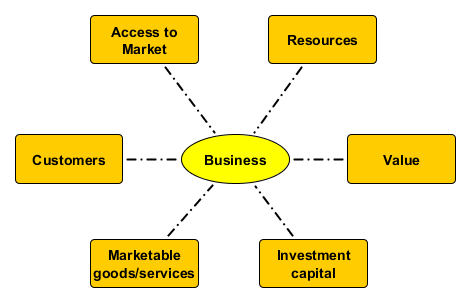
\includegraphics{images/keycomponents.png}
\caption{Key components of a thriving business}
\end{figure}

\hypertarget{essentials-of-business}{%
\section{Essentials of Business}\label{essentials-of-business}}

Business is a set of interactions in which goods and services are provided and compensation is rendered. Businesses become sustainable when the compensation rendered meets the short-term and long-term requirements of the business. Most business fail because of an inability to develop a network of processes and transactions to address a market demand that meets or exceeds their expenses. Ideally, a start-up should aim to seek fair compensation for goods and services rendered in the most effective and efficient manner.

\BeginKnitrBlock{rmdexercise}
\textbf{Exercise: The Nature of Business}

Discuss how the following premises would impact the nature, as well as the potential for long-term success of businesses.

\begin{enumerate}
\def\labelenumi{\arabic{enumi}.}
\tightlist
\item
  Business is all about making lots and lots of money quickly by any means possible.
\item
  Business is about fair compensation for goods and service to both suppliers and customers.
\item
  Business is the process of copying the industry leaders to provide similar goods and services at a fraction of the cost.
\item
  Business provides special opportunities for myself, my friends and relatives at the expense of our customers.
\end{enumerate}
\EndKnitrBlock{rmdexercise}

\hypertarget{business-processes}{%
\subsection{Business processes}\label{business-processes}}

Individual businesses are always centered around a core set of goods and services which address the specific needs of clients creating a sense of value and desire. Good design and pre-market testing help to define the nature of the products and services. At the same time, controlling production and distribution costs make it possible to deliver goods and services at a suitable price point for customers. Careful supply chain and operations management develops a network of contracts and business transactions with suppliers and distributors ensures that products and services are delivered on time and on budget.

\begin{figure}
\centering
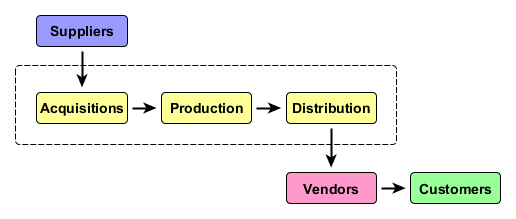
\includegraphics{images/businessprocess.png}
\caption{Key Business Processes}
\end{figure}

\BeginKnitrBlock{rmdexercise}
\textbf{Exercise: Match market principles to market characteristics}

\begin{longtable}[]{@{}ll@{}}
\toprule
\begin{minipage}[b]{0.44\columnwidth}\raggedright
Principles\strut
\end{minipage} & \begin{minipage}[b]{0.50\columnwidth}\raggedright
Characteristics\strut
\end{minipage}\tabularnewline
\midrule
\endhead
\begin{minipage}[t]{0.44\columnwidth}\raggedright
(A) Access to market \newline(B) Brand recognition\newline (C) Customer pool\newline(D) Investment capital\newline(E) Resources\newline(F) Market value\strut
\end{minipage} & \begin{minipage}[t]{0.50\columnwidth}\raggedright
\_\_\_ Consumer preference\newline  \_\_\_ Supply of raw materials\newline \_\_\_ Distinctive goods and services\newline\_\_\_ Investors and stock holders\newline \_\_\_ Location and traffic\newline\_\_\_ Steady market demand\strut
\end{minipage}\tabularnewline
\bottomrule
\end{longtable}
\EndKnitrBlock{rmdexercise}

\hypertarget{core-activities-of-a-business}{%
\subsection{Core Activities of a Business}\label{core-activities-of-a-business}}

Business requires coordinated teamwork of specialists in various departments to achieve efficiency and effectiveness on a large scale.

\begin{itemize}
\tightlist
\item
  \textbf{Finance:} mid-term and long-range financial planning to ensure that there is an adequate supply of money available to
\item
  \textbf{Accounting:} a record of financial commitments and compensations for the purpose of tracking movement of value across the organization and throughout the production process
\item
  \textbf{Marketing:} getting groups of potential customers and consumers interested in products and services.
\item
  \textbf{Sales:} selling products and services to customers maintain records to assist forecasting future demand and market growth
\item
  \textbf{Operations:} systems to acquire resources, produce, package and deliver products
\item
  \textbf{Management:} sets the direction and pace of business endeavors
\end{itemize}

\hypertarget{support-functions}{%
\subsection{Support functions}\label{support-functions}}

As businesses grow in size, various support functions are required to keep the core business running. These functions include the following:

\begin{itemize}
\tightlist
\item
  \textbf{Management Information Systems:} collect, analyze and distribute mission-critical information to key administrators
\item
  \textbf{Human Resources:} attract, hire, train and retain effective employees
\item
  \textbf{Legal Department:} ensure compliance with laws and regulations
\item
  \textbf{Investor Relations:} communications with shareholders to attract support and investments
\item
  \textbf{Customer Relations:} after sales care of customers and encouragement of brand loyalty
\item
  \textbf{Facilities Management:} maintenance of facilities and equipment to maximize the utility and value of capital investments in equipment and infrastructure.
\end{itemize}

\BeginKnitrBlock{rmdexercise}
\textbf{Exercise: Key business concepts}

Create a mindmap that illustrates the relationship between the following sets of terms, along with their Thai translations.

\begin{itemize}
\tightlist
\item
  \textbf{Key business components:} Access to market; Resources; Value; Investment capital; Marketable goods and services; Customers
\item
  \textbf{Core business activities:} Finance; Accounting; Marketing; Sales; Operations; Management.
\item
  \textbf{Support functions:} Management information systems; Human resources; Legal department; Investor relations; Customer relations; Facilities management
\end{itemize}
\EndKnitrBlock{rmdexercise}

\hypertarget{understanding-the-role-of-it-in-business}{%
\section{Understanding the role of IT in business}\label{understanding-the-role-of-it-in-business}}

As IT Departments become integrated into the business strategy, they provide tools, information and communication systems that can play a transformative role in the nature of the business. Enterprise Architecture tend to grow as IT Department move along these evolutionary steps. \citep{Hohpe2017a}, \citep{Hohpe2017b}

\hypertarget{the-establishment-of-an-it-department}{%
\subsection{The Establishment of an IT Department}\label{the-establishment-of-an-it-department}}

\begin{enumerate}
\def\labelenumi{\arabic{enumi}.}
\tightlist
\item
  Understand the business strategy
\item
  Translate into an IT strategy
\item
  Create transparency for IT developments
\item
  Define IT target picture
\item
  Define the roadmap for implementing IT
\item
  Harmonize and govern
\item
  Obtain feedback and refine
\item
  Coach and mentor
\end{enumerate}

Among IT Managers, there appears to be 2 major approaches to understanding the nature of business and IT's function: using IT to redesign the business or engineering the current organization. The political implications of the approach chosen can be immense and often the success of an IT manager will depend on the level of support from those that manage the IT department manager.

\begin{longtable}[]{@{}ll@{}}
\toprule
Architecting the Business & Reverse-Engineering the Organization\tabularnewline
\midrule
\endhead
* Identification of growth areas & * Divisions and business lines\tabularnewline
* Profitability of goods and services & * Group level vs divisions\tabularnewline
* Geographic/demographic opportunities & * Reportings lines\tabularnewline
* Geopolitical aspects & * Matrix organizations\tabularnewline
* Acquisitions and divestitures & * Hidden org chart/loyalties\tabularnewline
\bottomrule
\end{longtable}

\hypertarget{business-views-of-the-role-of-it}{%
\subsection{Business views of the role of IT}\label{business-views-of-the-role-of-it}}

Business managers have 4 main approaches to managing IT based on the main focus of the business administration.

\begin{longtable}[]{@{}rcclc@{}}
\toprule
\textbf{Focus} & \textbf{Role} & \textbf{Reports to} & \textbf{Common stragegy} & \textbf{Levers}\tabularnewline
\midrule
\endhead
Cost of IT & Cost Center & CFO & Outsource IT & Cost cutting\tabularnewline
Return on investment & Asset & COO & Harmonize / Rationalize & Economies of scale\tabularnewline
Business value of IT & Partner & CDO & Insource IT & Economies of Efficiency\tabularnewline
Speed / innovation & Enabler & CEO & IT = business & Economies of Speed\tabularnewline
\bottomrule
\end{longtable}

IT Strategy provides a road map of where IT developments and operations are going. This is derived from an understanding of the nature of the business and is not restricted by current realities. The IT strategy is as much a definition of what IT intends to do as well as what it will not do. Above all, an effective IT Business strategy does not conform to a vendor's product road map. However, successful strategies must recognize the IT Operating Model that the business gives to IT. \citep{Ross2006}

\textbf{IT Operating Models}

\begin{longtable}[]{@{}cll@{}}
\toprule
\begin{minipage}[b]{0.14\columnwidth}\centering
Integration\strut
\end{minipage} & \begin{minipage}[b]{0.45\columnwidth}\raggedright
Minimal Standards\strut
\end{minipage} & \begin{minipage}[b]{0.32\columnwidth}\raggedright
Highly Standardized\strut
\end{minipage}\tabularnewline
\midrule
\endhead
\begin{minipage}[t]{0.14\columnwidth}\centering
High\strut
\end{minipage} & \begin{minipage}[t]{0.45\columnwidth}\raggedright
\textbf{Coordination}\strut
\end{minipage} & \begin{minipage}[t]{0.32\columnwidth}\raggedright
\textbf{Unification}\strut
\end{minipage}\tabularnewline
\begin{minipage}[t]{0.14\columnwidth}\centering
\strut
\end{minipage} & \begin{minipage}[t]{0.45\columnwidth}\raggedright
* Unique business units* Examples: Merrill Lynch, Toyota* Key IT capability:~~ - access to shared data~~ - standard technology interfaces\strut
\end{minipage} & \begin{minipage}[t]{0.32\columnwidth}\raggedright
* Single business with global standards* Examples: Delta Airlines, Pepsi* Key IT capability:~~ - enterprise systems to reinforce standards~~- provide access to global data\strut
\end{minipage}\tabularnewline
\begin{minipage}[t]{0.14\columnwidth}\centering
Low\strut
\end{minipage} & \begin{minipage}[t]{0.45\columnwidth}\raggedright
\textbf{Diversification}\strut
\end{minipage} & \begin{minipage}[t]{0.32\columnwidth}\raggedright
\textbf{Replication}\strut
\end{minipage}\tabularnewline
\begin{minipage}[t]{0.14\columnwidth}\centering
\strut
\end{minipage} & \begin{minipage}[t]{0.45\columnwidth}\raggedright
* Independent business units * different customers/expertise * Examples: Johnson \& Johnson, GE * Key IT capability:~~ - provide economies of scale ~~ - do not limit independence\strut
\end{minipage} & \begin{minipage}[t]{0.32\columnwidth}\raggedright
* Independent but similar business units* Example: Marriott, CEMEX* Key IT capability:~~ - provide standard infrastructure and app~~ - maximize global efficiencies\strut
\end{minipage}\tabularnewline
\bottomrule
\end{longtable}

\hypertarget{software-to-facilitate-business-interactions}{%
\subsection{Software to facilitate business interactions}\label{software-to-facilitate-business-interactions}}

As a business grows, so does the complexity of the interactions between its departments. There is a complex web of interactions within a modern business organization. Management focuses on the control, operation, and development of a business. Financiers use investments to maximize opportunities to grow the business. Production engineers tune the processes needed to deliver products, But the key concern for IT is the nature and volume of information to be analyzed, shared and communicated in a timely fashion,
as shown in the following diagram:

\begin{figure}
\centering
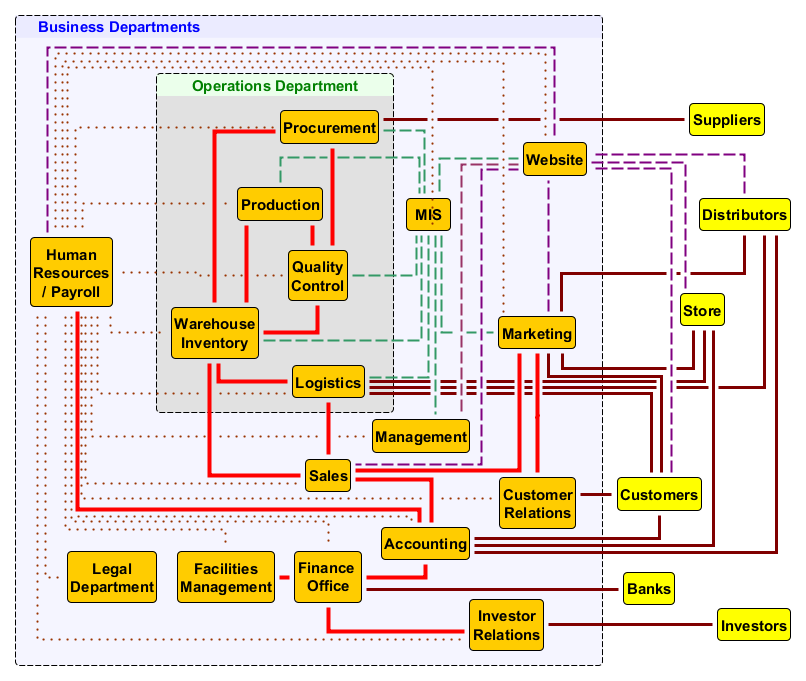
\includegraphics{images/businessdepts.png}
\caption{Interactions between business departments}
\end{figure}

Even with over 50 years of intensive development to reduce the complexity of doing business, new software tools and apps are still emerging at an astounding rate. The following sidebars attempt to classify common software systems found in medium to large size enterprises into 2 basic types of business systems.

\begin{itemize}
\item
  \textbf{Enterprise Resource Planning (ERP):} data systems that store and communicate operational data in a way facitates reporting and future planning.
\item
  \textbf{Enterprise Resource Management (ERM):} software systems that facilitate the monitor and manage interaction and the use of resources.
\end{itemize}

\BeginKnitrBlock{rmdextra}
\hypertarget{erp-software-systems}{%
\section*{ERP Software Systems}\label{erp-software-systems}}
\addcontentsline{toc}{section}{ERP Software Systems}

\begin{itemize}
\item
  \textbf{CONTENT MANAGEMENT SYSTEM (CMS):}

  \begin{itemize}
  \tightlist
  \item
    Collections of guides, rulebooks, forms, and procedure guidelines
  \item
    Blogs, newsletter, announcements
  \item
    Catalogues, price lists
  \item
    Documentation of intellectual property and licenses
  \end{itemize}
\item
  \textbf{PRODUCT INFORMATION MANAGEMENT (PIM):}

  \begin{itemize}
  \tightlist
  \item
    Manual, troubleshooting guides
  \item
    Parts list, equivalences
  \item
    Price lists and stock inventory
  \item
    Photos and promotional materials
  \end{itemize}
\item
  \textbf{Accounting Information System (AIS):}

  \begin{itemize}
  \tightlist
  \item
    Revenue: cash inflow (sales)
  \item
    Expenditure: cash outflow (payroll, equipment)
  \item
    Conversion: work-in-progress transactions (raw material, precursor inventory)
  \item
    Administrative: reporting (income statement, balance sheet, cash flows)
  \end{itemize}
\end{itemize}
\EndKnitrBlock{rmdextra}

\BeginKnitrBlock{rmdextra}
\hypertarget{erm-software-systems}{%
\section*{ERM Software systems}\label{erm-software-systems}}
\addcontentsline{toc}{section}{ERM Software systems}

\begin{itemize}
\item
  \textbf{B2B: Business-to-business software:} manages workflow with suppliers and partners

  \begin{itemize}
  \tightlist
  \item
    Directory of suppliers and products
  \item
    Social media confirmation of quality
  \end{itemize}
\item
  \textbf{B2C: Business-to-consumer software:} serve the needs of individual customers particularly in regards to customer history, order status, and billing information.

  \begin{itemize}
  \tightlist
  \item
    Online store
  \item
    Product manuals, product information
  \item
    Delivery tracking
  \end{itemize}
\item
  \textbf{Human Resources Management (HRM):}

  \begin{itemize}
  \tightlist
  \item
    Payroll, bonuses, raises
  \item
    Staff work experience, Performance appraisal, skill tests
  \item
    Flight risk, employee satisfaction
  \item
    Education, training
  \end{itemize}
\item
  \textbf{Marketing Automation Platform (MAP):}

  \begin{itemize}
  \tightlist
  \item
    CRM: Customer Relationship Management - purchase history, rewards, interests,
  \item
    MCP: Marketing Campaign Planning - Ad words, analytics, costs, contracts, effectiveness
  \end{itemize}
\end{itemize}
\EndKnitrBlock{rmdextra}

\hypertarget{essentials-of-business-quality-management}{%
\section{Essentials of Business Quality Management}\label{essentials-of-business-quality-management}}

Businesses are driven by an active communication chain that drives the business process. The effectiveness of teamwork and management depends on effective communication. However, the communication chain can be interrupted by bottlenecks in the flow of data, inconsistent or misleading reporting, and other communication breakdowns. Quality standards help ensure that processes related to production and quality control are subject to timely, data-driven management. In essence the ability of a business to fix a problem depends on the quality of communications that provide access to the description of the true nature and extend of the problem and knowledge of possible remedies.

\begin{figure}
\centering
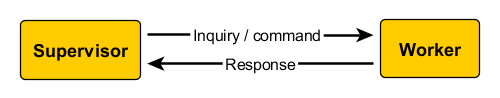
\includegraphics{images/communication.png}
\caption{Communication Chain}
\end{figure}

Meaningful communication requires a reciprocal interaction between the speaker and the listener. As shown in the following table, social norms and good ethicate depend on transmission of a message and an appropriate response. The communication chain is lost when messages in either direction are lost or misinterpreted. The growing use of social media with its emphasis on icons or one word responses has often been blamed for the reduction in quality of personal verbal and written skills. Interaction with customers and suppliers depends on clear and effective communication.

\begin{longtable}[]{@{}ll@{}}
\toprule
Initiation message & Response message\tabularnewline
\midrule
\endhead
Greeting & Acknowledgement\tabularnewline
Question & Response\tabularnewline
Proposal & Acceptance/Rejection\tabularnewline
Command & Action\tabularnewline
Accusation & Acceptance/Rebuttal\tabularnewline
\bottomrule
\end{longtable}

\hypertarget{iso9000iso9001}{%
\subsection{ISO9000/ISO9001}\label{iso9000iso9001}}

ISO 9000 was first published in 1987 by the International Organization for Standardization (ISO). The derivative quality standards help organizations address the needs of customers and while meeting relevant statutory and regulatory requirements.\citep{ISOweb} The ISO9001 standards provide guidance and tools for companies and organizations who want to ensure that their processes regularly deliver products and services that meet customer's requirements. It also defines the requirements for certification against these standards which are reviewed and revised every 5 years.\citep{ISO2015}

\begin{itemize}
\tightlist
\item
  \textbf{Point 1: Clear customer understanding} of the goods or services offered within a business contract.
\item
  \textbf{Point 2: Verification of intended results} to ensure that the terms of the business contract were met.
\item
  \textbf{Point 3: Prevention of undesired effects} that might cause delays or problems in the delivery of goods and services
\item
  \textbf{Point 4: Improve performance} based on the information gathered
\end{itemize}

\BeginKnitrBlock{rmddiscussion}
\textbf{An example of an ISO9001 compliant transaction}

Discuss what points of the ISO9001 standard is satisfied by the follow stages of a simple business transaction at a restuarant.

\begin{enumerate}
\def\labelenumi{\arabic{enumi}.}
\tightlist
\item
  The customer enters a restaurant and is given a menu with pictures of the food.
\item
  The waiter takes the order and repeats the order back to the customer for confirmation.
\item
  The waiter brings the food and doubles check that the order is complete.
\item
  The waiter comes back to check if everything is okay.
\item
  The cashier checks that all was well when the bill is paid.
\item
  The whole transaction is recorded and the receipt gives a website for feedback.
\item
  The customer's feedback on the website is analyzed for patterns of service that could be improved.
\end{enumerate}
\EndKnitrBlock{rmddiscussion}

\BeginKnitrBlock{rmdexercise}
\textbf{Exercise: ISO9001 and MacDonalds}

Worldwide MacDonald is a successful multinational enterprise run by staff most of which are under the age of 21 and yet it is a certified ISO9001 company. When a customer orders food at any MacDonald outlet in the world, the interaction between the customer and the counter staff is always the same.

\begin{itemize}
\tightlist
\item
  Create a swim lane workflow diagram to describe the information flow in the conversation between the customer, the counter staff, the kitchen staff, the accounting system, and the point-of-sale computer system.
\item
  Identify how the basic principles of ISO9001 principles for quality management are a ddressed by this basic operating procedure..
\end{itemize}
\EndKnitrBlock{rmdexercise}

\hypertarget{changes-to-business}{%
\section{Changes to Business}\label{changes-to-business}}

Businesses today have unprecedented opportunities to rapidly address issues that arise. Such advances in such fields as deep machine learning, Big Data analytics, Internet of Things, collective intelligence, online payment and social media are creating a reality that was only hinted at by the 1999 book \textbf{\emph{Business at the speed of thought.}} \citep{Gates1999} Businesses that were market leaders in the past, but failed to keep pace with the changes, suddenly find themselves bankrupt and replaced by new competitors. In 500BC, Heraclitus of Ephesus once penned the warning that ``Change is the only constant in life'' but he words ring true as an accurate description of today's business environment.

\hypertarget{open-organization}{%
\subsection{Open Organization}\label{open-organization}}

Since ISO9000 was first published in 1987, it has been revised and replaced by a long list of international standards that define and specify how various aspects of business, hardware, and software are to be implemented. Each new standard built on the principles already established and addresses the weaknesses of previous standards. \citep{ISO2015} While these developments help to ensure consistent service and quality, something else was needed to empower staff to collectively think and implement creative solutions to challenges. Jim Whitehurst at RedHat.com invested considerable effort to address this problem. He started with the realization that ``the best practices in creating open source software also translate well into managing an entire company.'' By embracing open source values and creating a new open standard for communities, he showed how leaders can successfully create ``a rebooted, redesigned, reinvented organization suitable for the decentralized, empowered, digital age.''\citep{Whitehurst2015} In creating the open organization, he and his colleagues have documented a shift that is changing in the way businesses are organized, managed and run.

\begin{longtable}[]{@{}ll@{}}
\toprule
\begin{minipage}[b]{0.47\columnwidth}\raggedright
Traditional values\strut
\end{minipage} & \begin{minipage}[b]{0.47\columnwidth}\raggedright
Post-Modern values\strut
\end{minipage}\tabularnewline
\midrule
\endhead
\begin{minipage}[t]{0.47\columnwidth}\raggedright
Loyality to the organizational hierachy\strut
\end{minipage} & \begin{minipage}[t]{0.47\columnwidth}\raggedright
Loyality to the mission, purpose and values of the company\strut
\end{minipage}\tabularnewline
\begin{minipage}[t]{0.47\columnwidth}\raggedright
Compliance\strut
\end{minipage} & \begin{minipage}[t]{0.47\columnwidth}\raggedright
Focus creativity to create solutions\strut
\end{minipage}\tabularnewline
\begin{minipage}[t]{0.47\columnwidth}\raggedright
Predictability\strut
\end{minipage} & \begin{minipage}[t]{0.47\columnwidth}\raggedright
Adaptability to change\strut
\end{minipage}\tabularnewline
\begin{minipage}[t]{0.47\columnwidth}\raggedright
Efficiency\strut
\end{minipage} & \begin{minipage}[t]{0.47\columnwidth}\raggedright
Effectiveness\strut
\end{minipage}\tabularnewline
\begin{minipage}[t]{0.47\columnwidth}\raggedright
Plan, Prescribe, Execute\strut
\end{minipage} & \begin{minipage}[t]{0.47\columnwidth}\raggedright
Envision, Prioritize, Implement, Adjust\strut
\end{minipage}\tabularnewline
\bottomrule
\end{longtable}

Successful, innovative organizations demonstrate the following core principles which form the basis for the core elements of open organizations. \citep{Whitehurst2019}

\begin{itemize}
\tightlist
\item
  The best ideas come from anywhere.
\item
  The best ideas should always win.
\item
  Contribution matters more than title.
\end{itemize}

\begin{figure}
\centering
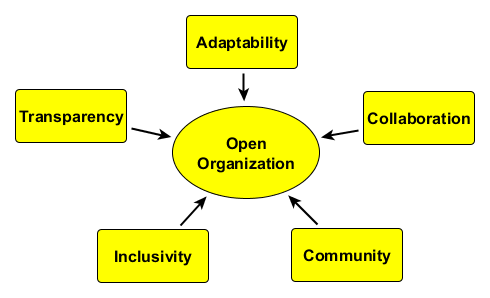
\includegraphics{images/openorg.png}
\caption{Core elements of open organizations}
\end{figure}

Although every open organization is unique, there is a common core of elements that characterize open organizations. Each core element is composed of a different dataset to be gathered, distributed, and combined in powerful and productive ways.

\begin{itemize}
\tightlist
\item
  \textbf{Transparency:} Workers have access to all pertinent information and willingly disclose and discuss their work. Workers can access and review the processes and arguments that lead to decisions and are free to comment and respond to them. Successes and failures are valued for the lessons they provide.
\item
  \textbf{Inclusivity:} Protocols and procedures are developed to encourage constructive discussion from diverse perspectives. Leaders actively seek to include voices not present in the dialog. Technology is used to ensure and encourage access to discussion forums.
\item
  \textbf{Adaptability:} Feedback mechanisms provide access for suggestions from members of the organizations and outside members.
\item
  \textbf{Collaboration:} The organization adheres to the principle that working together produces better results. Products of development are made available to other projects to use creatively.
\item
  \textbf{Community:} Shared values and principles that guide decision making are clear and obvious to members of the organization. All workers are encouraged and empowered to make meaningful contributions to the collaborative effort. Leaders mentor others and model shared values and principles.
\end{itemize}

As organizations embrace the core concepts of open organizations, they discover that openness is necessary for success and that attempts to pursue openness will lead to 3 possible outcomes: \citep{OOA2017}

\begin{itemize}
\item
  \textbf{Greater agility:} resulting from the synergy that arises when members share a common vision and work together toward common goals.
\item
  \textbf{Faster innovation:} because ideas from both inside and outside the organization receive more equitable consideration and rapid experimentation
\item
  \textbf{Increased engagement:} as members clearly see connections between their particular activities and an organization's overarching values, mission, and spirit.
\end{itemize}

\BeginKnitrBlock{rmdextra}
\hypertarget{working-as-a-developer-within-an-open-organization}{%
\section*{Working as a developer within an open organization}\label{working-as-a-developer-within-an-open-organization}}
\addcontentsline{toc}{section}{Working as a developer within an open organization}

Increasingly large IT development center like Google, Oracle and Apple are becoming open organizations to encourage and value innovation. Each worker in those companies is expected to do his/her part in contributing to the development effort. However, young IT staff have a very high rate of turn over as they are often foreign to working in environments that productively focus creativity to solve issues. This mismatch was the inspiration behind a recent blog concerning the five laws that development engineers should know. \citep{Short2017}

\begin{enumerate}
\def\labelenumi{\arabic{enumi}.}
\tightlist
\item
  \textbf{Forget the phrase `I do not know':} Treat every task as an opportunity to learn and dedicate the time needed to become an expert
\item
  \textbf{Read the manual! :} Documentation was written for a purpose. Do not waste colleague's time.
\item
  \textbf{Search before asking:} Do not contribute to the problems but contribute to the solution.
\item
  \textbf{Anything is possible:} Anything is possible in this space with proper time, coordination, and effort. Trust by verifying new ideas
\item
  \textbf{Acknowledge technical debt:} Technical debt is the result of decisions that made sense at the time someone made them but cause problems because they are not based on reality.
\end{enumerate}
\EndKnitrBlock{rmdextra}

\hypertarget{the-changing-nature-of-customers}{%
\subsection{The changing nature of customers}\label{the-changing-nature-of-customers}}

Advances in technology have changed both the ability to produce product and the nature of markets. The internet and social media have exposed individuals to a wider range of products and vendors. This creates new desires and expectations in customers and increased competition among business. At the same time, social changes are impacting markets, particularly as youth explore new careers, lifestyles, technologies, and life goals.

\BeginKnitrBlock{rmdextra}
\textbf{Changing indicators of success in Singapore}

The most common indicators of success mentioned in conversation with Singapore voters in 2000 was compare to the list compiled from conversations with Singaporen youth in 2018. \citep{SNYCYC2019}, \citep{Tan2019}

\begin{longtable}[]{@{}rll@{}}
\toprule
Level & Traditional success indicators & Goals of Singapore Youth\tabularnewline
\midrule
\endhead
1 & Career / Work & Emotional well being\tabularnewline
2 & Finance / Money & Personal learning / Skill development\tabularnewline
3 & Studies / Degrees & Family\tabularnewline
4 & Family & Finance / Money\tabularnewline
5 & House / Belongings & Spirituality\tabularnewline
\bottomrule
\end{longtable}

\textbf{Top 10 Life Goals Important to Singapore Youth}

\begin{longtable}[]{@{}lr@{}}
\toprule
Goals & Percent\tabularnewline
\midrule
\endhead
Home ownership & 70\%\tabularnewline
Strong family relationships & 70\%\tabularnewline
Learning / acquiring new skils & 62\%\tabularnewline
Successful career & 59\%\tabularnewline
Earn lots of money & 46\%\tabularnewline
Help less fortunate & 41\%\tabularnewline
Contribute to society & 40\%\tabularnewline
Get married & 36\%\tabularnewline
Have children & 35\%\tabularnewline
Good religious life & 31\%\tabularnewline
\bottomrule
\end{longtable}
\EndKnitrBlock{rmdextra}

Today's businesses need to be as versatile and diverse as the customers and markets they serve. In the past, only businesses with a large customer base were about to benefit from economies of scale. However, online services have made it possible for businesses to support both mass distribution to millions of consumers while at the same time of catering to the diverse needs of individual customers that number in the millions.

\BeginKnitrBlock{rmddiscussion}
\textbf{Discussion: Impact of changes in life goals on business}

\begin{enumerate}
\def\labelenumi{\arabic{enumi}.}
\item
  How do you think changes in life goals of youth will impact the market place?
\item
  Based on these changes, which products would be expected to have the greatest increases or decreases in demand in the next 10 or 20 years?
\item
  What aspirations of Thai youth have changed in the last 10 years?
\item
  What impact will these changes have on the Thai economy?
\end{enumerate}
\EndKnitrBlock{rmddiscussion}

In addition, social media provide a forum for expressing opinions without being held accountable for the view expressed. Generally, the rewards for being liked help to regulate the web but increasing courts are given the power to litigate on defamation cases where rumors have caused damage. Nonetheless, social media continue to have an impact on Brand and Product Marketing,particularly in the following ways.

\begin{enumerate}
\def\labelenumi{\arabic{enumi}.}
\tightlist
\item
  Word-of-mouth referrals from trusted acquaintances are powerful endorsements and attractions.
\item
  Customer testimonials are often decisive in purchasing decisions.
\item
  Community discussion of the products being developed increases trust in the company.
\item
  False testimonies are a problem: fakes entries attempt to oversell a product or provide complaints in an attempt to destroy the company.
\item
  Online searches and discussions are becoming the primary source of information for most.
\end{enumerate}

\BeginKnitrBlock{rmddiscussion}
Given the changes in the nature of the online market, discuss how the following approaches help to target the population to focus on those who are most likely to purchase. For each of these approaches, identify the nature of a particular market for which it would be more effective than the others.

\begin{enumerate}
\def\labelenumi{\arabic{enumi}.}
\tightlist
\item
  Search engine ads based on topics being searched
\item
  Social media ads based on shared views and ideas
\item
  Personal profiling to drive the user experience at a website based on specific interests and preferences expressed
\end{enumerate}
\EndKnitrBlock{rmddiscussion}

\hypertarget{changing-nature-of-business}{%
\subsection{Changing nature of business}\label{changing-nature-of-business}}

It is clear that the retail companies in rapid growth are those who are able to upgrade the services of the traditional storefront into a more convenient, efficient and user-friendly setting that compliments the services available online. Banks have moved their services online and to ATM to increase the convenience of handling money while lowering operating costs. Online companies like Amazon have teamed up with traditional shopping chains like Target to allows customers the opportunity to compare, touch and feel products before purchasing them either in the shop or online. Online orders can be delivered to shops to reduce shipping costs. Amazon has even integrated such high tech features as AI, face recognition and sensor to change the user shopping experience.\citep{Amazon2016} Technology play a critical role in all of these developments.

\BeginKnitrBlock{rmddiscussion}
\hypertarget{new-generation-7-11-seven-eleven}{%
\section*{New generation 7-11 (Seven Eleven)}\label{new-generation-7-11-seven-eleven}}
\addcontentsline{toc}{section}{New generation 7-11 (Seven Eleven)}

View this news clip about a new Seven Eleven outlet that opened in Pattaya with a new look that is in keeping with the era of Thailand 4.0. The store is full of sensors, monitors and systems to create a modern, futuristic, efficient shopping and eating environment complete with innovations to improve energy-saving and user convenience. Watch the video \citep{Suriywong2018} and list the number of ways computers have been used to change the user experience.
\EndKnitrBlock{rmddiscussion}

\hypertarget{online-commerce}{%
\section{Online Commerce}\label{online-commerce}}

In 2019, it is estimated that over 56\% of the world's population has access to the internet. There are 26.6 billion devices and 4.39 billion people are connected to the internet. It is estimated that 3.48 billion social media users. Facebook alone has well over 2.36 billion users each month. Google answers 63,000 searches per second. This is creating unprecented levels of opportunity for marketing to huge markets world-wide. In the following graph, the number of users grows linearly while their revenues grow expotentally. \citep{Statista2019}

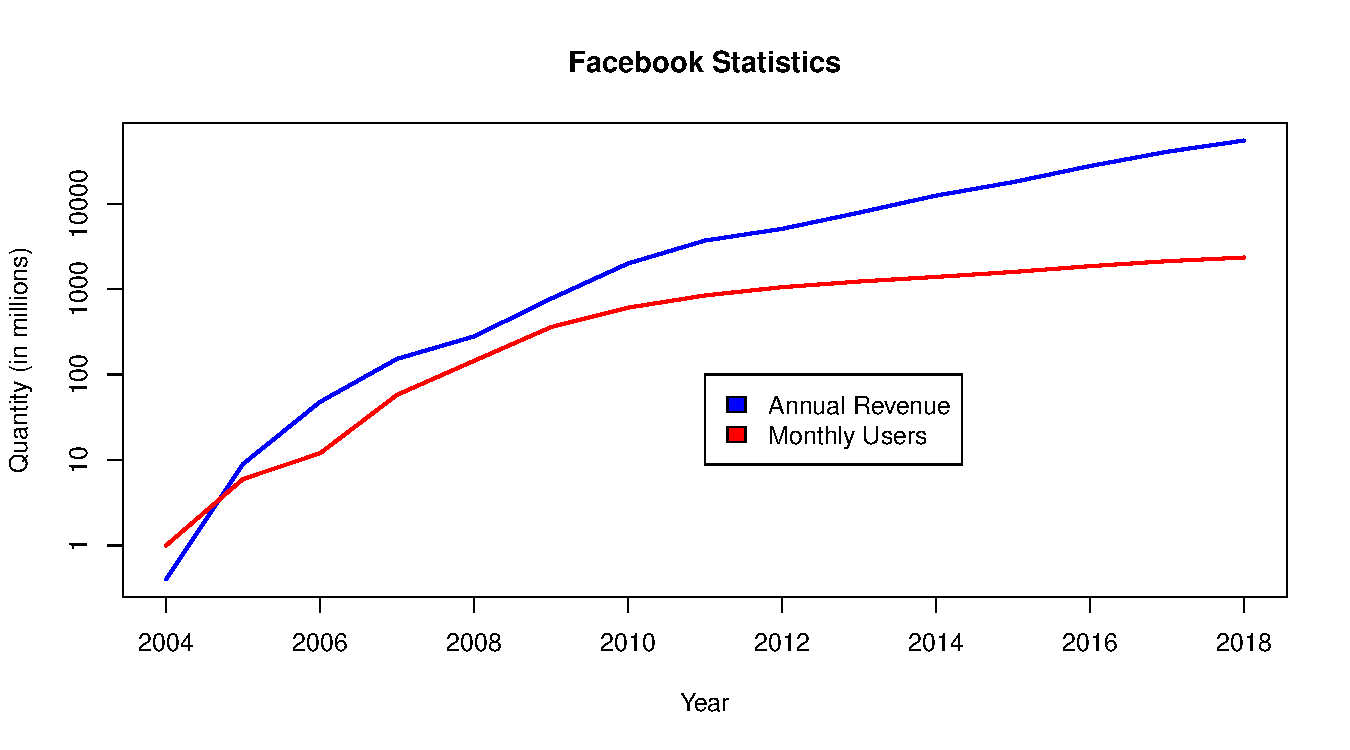
\includegraphics{bookdown-demo_files/figure-latex/unnamed-chunk-4-1.pdf}

\BeginKnitrBlock{rmddiscussion}
\textbf{The mobile phone market}
Review the statistics of the performance of leading mobile phone producers since 1994 {[}TNW2019{]} and discuss the following:

\begin{itemize}
\tightlist
\item
  What factors contributed to the fall of market leaders?
\item
  How will President Trump's technology embargo on China effect this market?
\item
  Is there room for new competitors in this market?
\end{itemize}
\EndKnitrBlock{rmddiscussion}

\hypertarget{growth-of-the-internet-and-e-commerce}{%
\subsection{Growth of the Internet and e-commerce}\label{growth-of-the-internet-and-e-commerce}}

As the following graph shows, the types of devices used to access the internet have also changed in the past decade.

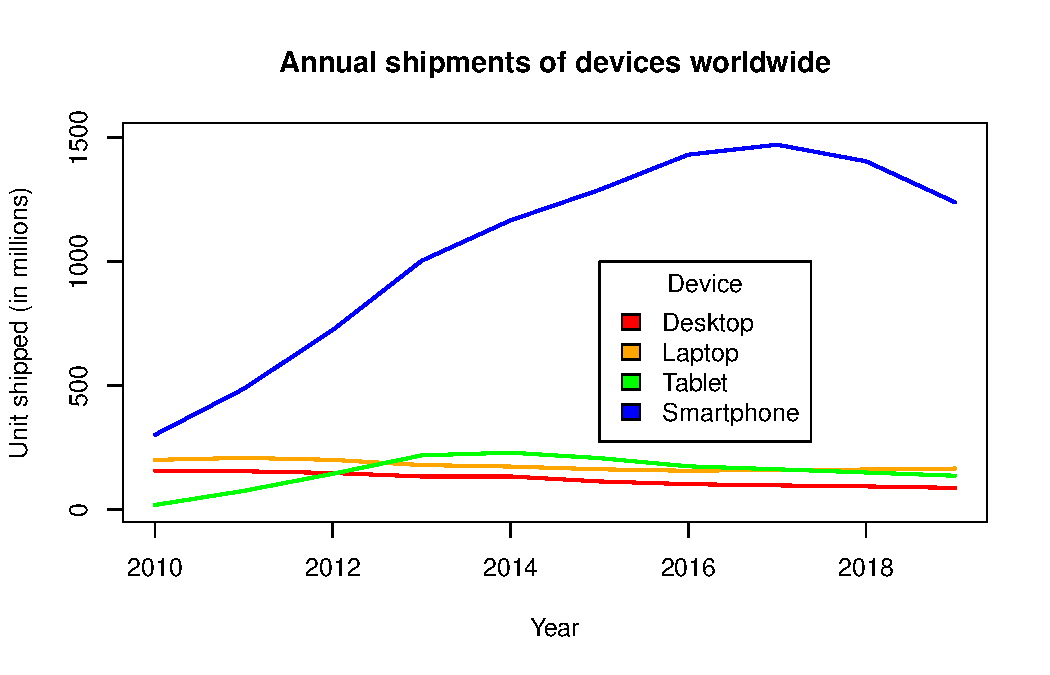
\includegraphics{bookdown-demo_files/figure-latex/unnamed-chunk-5-1.pdf}

The trend has been to using mobile devices for shopping, and surfing for possibilities. There appears to be some resistance to using mobile devices to order online.

\begin{longtable}[]{@{}rccc@{}}
\toprule
& Computer & Tablet & Smartphone\tabularnewline
\midrule
\endhead
E-commerce traffic & 53.9\% & 12.4\% & 33.7\%\tabularnewline
Volume of Retail sales & 76.9\% & 12.4\% & 10.7\%\tabularnewline
\bottomrule
\end{longtable}

With the development of the world wide web in the 1990s, online commerce has been gaining advantage over corresponding brick and mortar firms, especially for the following reasons:

\begin{enumerate}
\def\labelenumi{\arabic{enumi}.}
\tightlist
\item
  The customer has access to more information to make better purchasing decisions
\item
  The customer can shop 24x7
\item
  The customer can track the progress of order fulfillment.
\item
  Customers can find and provide feedback verified through social media.
\item
  The functions of e-commerce can be purchased and updated to keep development costs low and to maximize economies of scale
\end{enumerate}

However, the elderly are more resistant to adopt online shopping, but there is growing acceptance.

\textbf{Adoption of online shopping by age of internet user}

\begin{longtable}[]{@{}llllll@{}}
\toprule
Frequency & 18-29 & 30-39 & 40-49 & 50-64 & \textgreater{}65\tabularnewline
\midrule
\endhead
Once per week & 35\% & 37\% & 23\% & 17\% & 11\%\tabularnewline
Once per month & 41\% & 35\% & 35\% & 38\% & 31\%\tabularnewline
Once per year & 24\% & 28\% & 42\% & 45\% & 50\%\tabularnewline
Never & 0\% & 0\% & 0\% & 0\% & 8\%\tabularnewline
\bottomrule
\end{longtable}

\begin{figure}
\centering
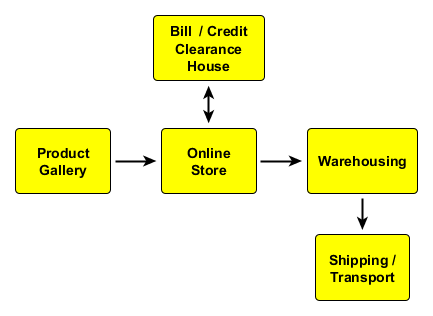
\includegraphics{images/ecommercefunctions.png}
\caption{Business Functions of E-Commerce}
\end{figure}

\hypertarget{the-e-shopping-customer-experience}{%
\subsection{The e-shopping customer experience}\label{the-e-shopping-customer-experience}}

As shown by the table below, The process of shopping for goods online has many similarities to shopping at traditional brick and mortar shops. These similarities have contributed to rapid growth in online purchases which in 2018 totaled \$2,489 trillion worldwide. This represents about 8.8\% of all sales worldwide. \citep{Saleh2019}

\begin{longtable}[]{@{}lll@{}}
\toprule
\begin{minipage}[b]{0.15\columnwidth}\raggedright
Stage\strut
\end{minipage} & \begin{minipage}[b]{0.38\columnwidth}\raggedright
Brick and Mortar\strut
\end{minipage} & \begin{minipage}[b]{0.38\columnwidth}\raggedright
Electronic world\strut
\end{minipage}\tabularnewline
\midrule
\endhead
\begin{minipage}[t]{0.15\columnwidth}\raggedright
Customer finds the store.\strut
\end{minipage} & \begin{minipage}[t]{0.38\columnwidth}\raggedright
Ads and billboards\strut
\end{minipage} & \begin{minipage}[t]{0.38\columnwidth}\raggedright
Google and Facebook Ads; Referrals from blogs\strut
\end{minipage}\tabularnewline
\begin{minipage}[t]{0.15\columnwidth}\raggedright
Customer shops for items of interest\strut
\end{minipage} & \begin{minipage}[t]{0.38\columnwidth}\raggedright
Window shopping\strut
\end{minipage} & \begin{minipage}[t]{0.38\columnwidth}\raggedright
Search the website\strut
\end{minipage}\tabularnewline
\begin{minipage}[t]{0.15\columnwidth}\raggedright
Customer searches for information on the products\strut
\end{minipage} & \begin{minipage}[t]{0.38\columnwidth}\raggedright
Check packaging and sales staff\strut
\end{minipage} & \begin{minipage}[t]{0.38\columnwidth}\raggedright
Internet searches and social media recommendations\strut
\end{minipage}\tabularnewline
\begin{minipage}[t]{0.15\columnwidth}\raggedright
Customer chooses items for purchase\strut
\end{minipage} & \begin{minipage}[t]{0.38\columnwidth}\raggedright
Places them in a cart or shopping basket\strut
\end{minipage} & \begin{minipage}[t]{0.38\columnwidth}\raggedright
Virtual transfer of items to an electronic shopping cart\strut
\end{minipage}\tabularnewline
\begin{minipage}[t]{0.15\columnwidth}\raggedright
Customer checkouts the selected items for purchase\strut
\end{minipage} & \begin{minipage}[t]{0.38\columnwidth}\raggedright
The customer takes the shopping cart to the check out counter\strut
\end{minipage} & \begin{minipage}[t]{0.38\columnwidth}\raggedright
The virtual cart is checked out creating a preliminary bill complete with shipping information\strut
\end{minipage}\tabularnewline
\begin{minipage}[t]{0.15\columnwidth}\raggedright
The financial institution identifies and authenticates the payer\strut
\end{minipage} & \begin{minipage}[t]{0.38\columnwidth}\raggedright
The customer swipes a credit card or ATM card\strut
\end{minipage} & \begin{minipage}[t]{0.38\columnwidth}\raggedright
The customer logs into to e-banking, e-payment or credit card services\strut
\end{minipage}\tabularnewline
\begin{minipage}[t]{0.15\columnwidth}\raggedright
The customer transfers funds to the vendor.\strut
\end{minipage} & \begin{minipage}[t]{0.38\columnwidth}\raggedright
The customer signs the electronic receipt or pays cash\strut
\end{minipage} & \begin{minipage}[t]{0.38\columnwidth}\raggedright
The customer verifies and authorizes payment\strut
\end{minipage}\tabularnewline
\begin{minipage}[t]{0.15\columnwidth}\raggedright
The financial institution send payment verification.\strut
\end{minipage} & \begin{minipage}[t]{0.38\columnwidth}\raggedright
ATM or Credit card service authenticates the transaction or the cashier\strut
\end{minipage} & \begin{minipage}[t]{0.38\columnwidth}\raggedright
The financial institution sends a secure memo to the e-store that payment was made.\strut
\end{minipage}\tabularnewline
\begin{minipage}[t]{0.15\columnwidth}\raggedright
The vendor sends a pick-list order to the fulfillment center.\strut
\end{minipage} & \begin{minipage}[t]{0.38\columnwidth}\raggedright
The storekeeper faxes the order to the warehouse\strut
\end{minipage} & \begin{minipage}[t]{0.38\columnwidth}\raggedright
The fulfillment center is notified of the order and its payment and picks the items\strut
\end{minipage}\tabularnewline
\begin{minipage}[t]{0.15\columnwidth}\raggedright
The fulfillment center sends the goods to the shipper.\strut
\end{minipage} & \begin{minipage}[t]{0.38\columnwidth}\raggedright
The items are boxed and set aside for pickup\strut
\end{minipage} & \begin{minipage}[t]{0.38\columnwidth}\raggedright
The items are boxed and sent to the shipper.\strut
\end{minipage}\tabularnewline
\begin{minipage}[t]{0.15\columnwidth}\raggedright
The fulfillment center updates the order status.\strut
\end{minipage} & \begin{minipage}[t]{0.38\columnwidth}\raggedright
The customer is called to pick up his order.\strut
\end{minipage} & \begin{minipage}[t]{0.38\columnwidth}\raggedright
The online system is updated and the customer can track its location.\strut
\end{minipage}\tabularnewline
\begin{minipage}[t]{0.15\columnwidth}\raggedright
The shipper delivers the goods.\strut
\end{minipage} & \begin{minipage}[t]{0.38\columnwidth}\raggedright
The counter staff check the delivery items and turns them over to the customer.\strut
\end{minipage} & \begin{minipage}[t]{0.38\columnwidth}\raggedright
The shipper delivers the goods.\strut
\end{minipage}\tabularnewline
\begin{minipage}[t]{0.15\columnwidth}\raggedright
The customer takes possession of the goods.\strut
\end{minipage} & \begin{minipage}[t]{0.38\columnwidth}\raggedright
The customer picks up the bags and leaves\strut
\end{minipage} & \begin{minipage}[t]{0.38\columnwidth}\raggedright
The customer signs for the goods and the tracking system is updated.\strut
\end{minipage}\tabularnewline
\bottomrule
\end{longtable}

\BeginKnitrBlock{rmddiscussion}
\hypertarget{hybrid-businesses}{%
\section{Hybrid businesses}\label{hybrid-businesses}}

Online shopping giant Amazon has recently merged with Target a traditional department store chain. Explain why this merger is a good idea and what benefits the customer gains from it.
\EndKnitrBlock{rmddiscussion}

\bibliography{book.bib,packages.bib}


\end{document}
